\section{Masse und Schwerpunktslage}

\newcommand{\hi}{{\textnormal{hinten}}}
\newcommand{\vo}{{\textnormal{vorne}}}
\newcommand{\li}{{\textnormal{links}}}
\newcommand{\re}{{\textnormal{rechts}}}
\newcommand{\gr}{{\textnormal{ g}}}
\newcommand{\m}{{\textnormal{ m}}}
\newcommand{\Abb}{\textbf{ABBILDUNG }}

\begin{figure}[h]
\centering
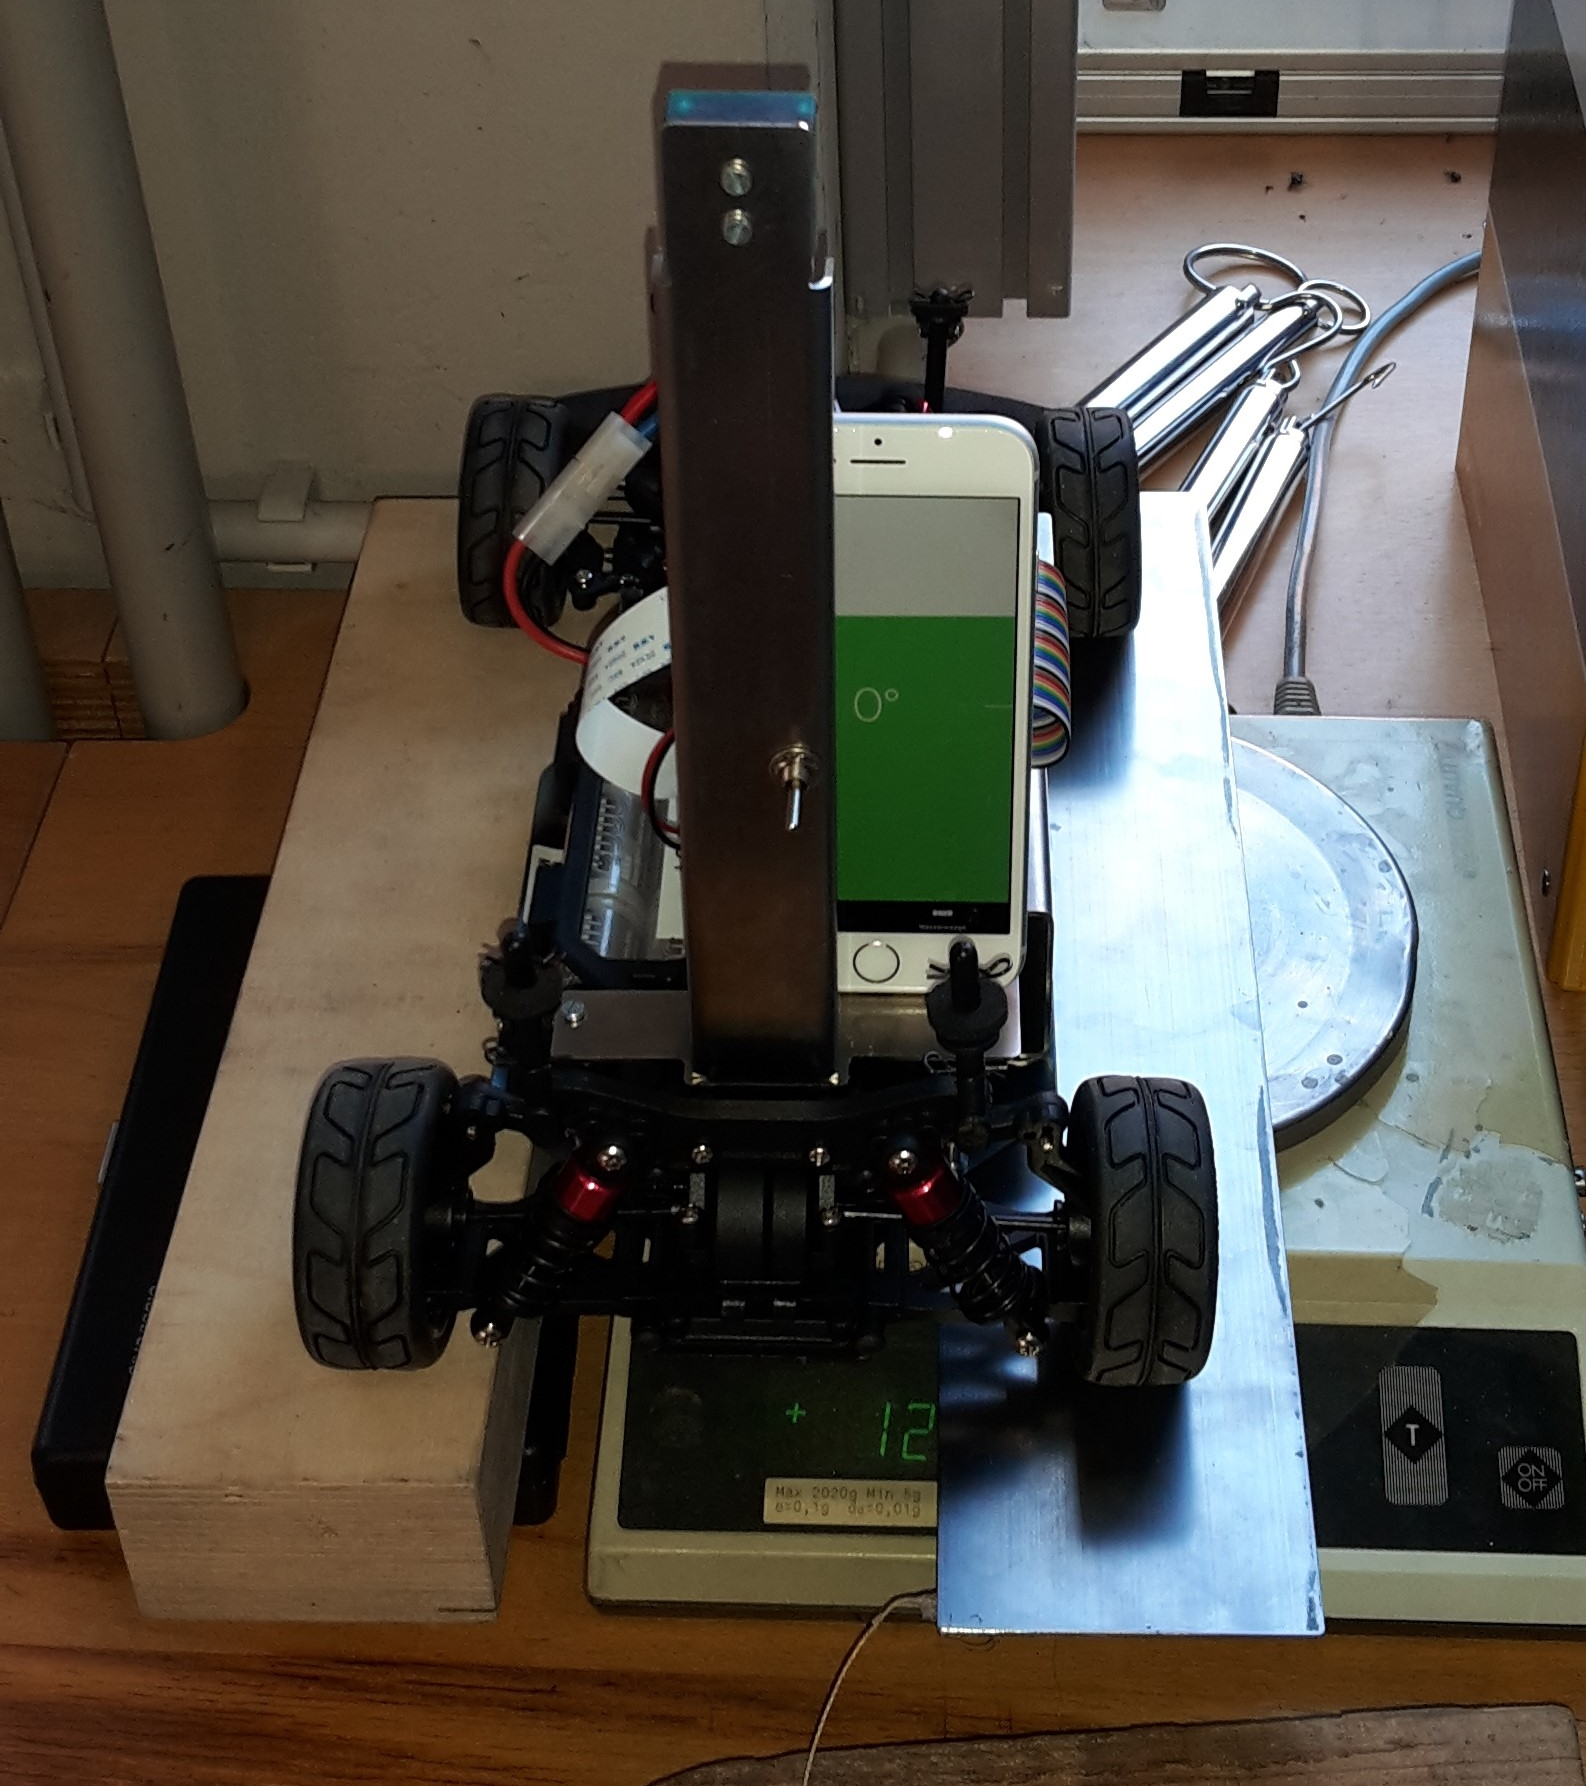
\includegraphics[width=0.3\textwidth]{Figures/Schwerpunktmessung_links_rechts.jpg}
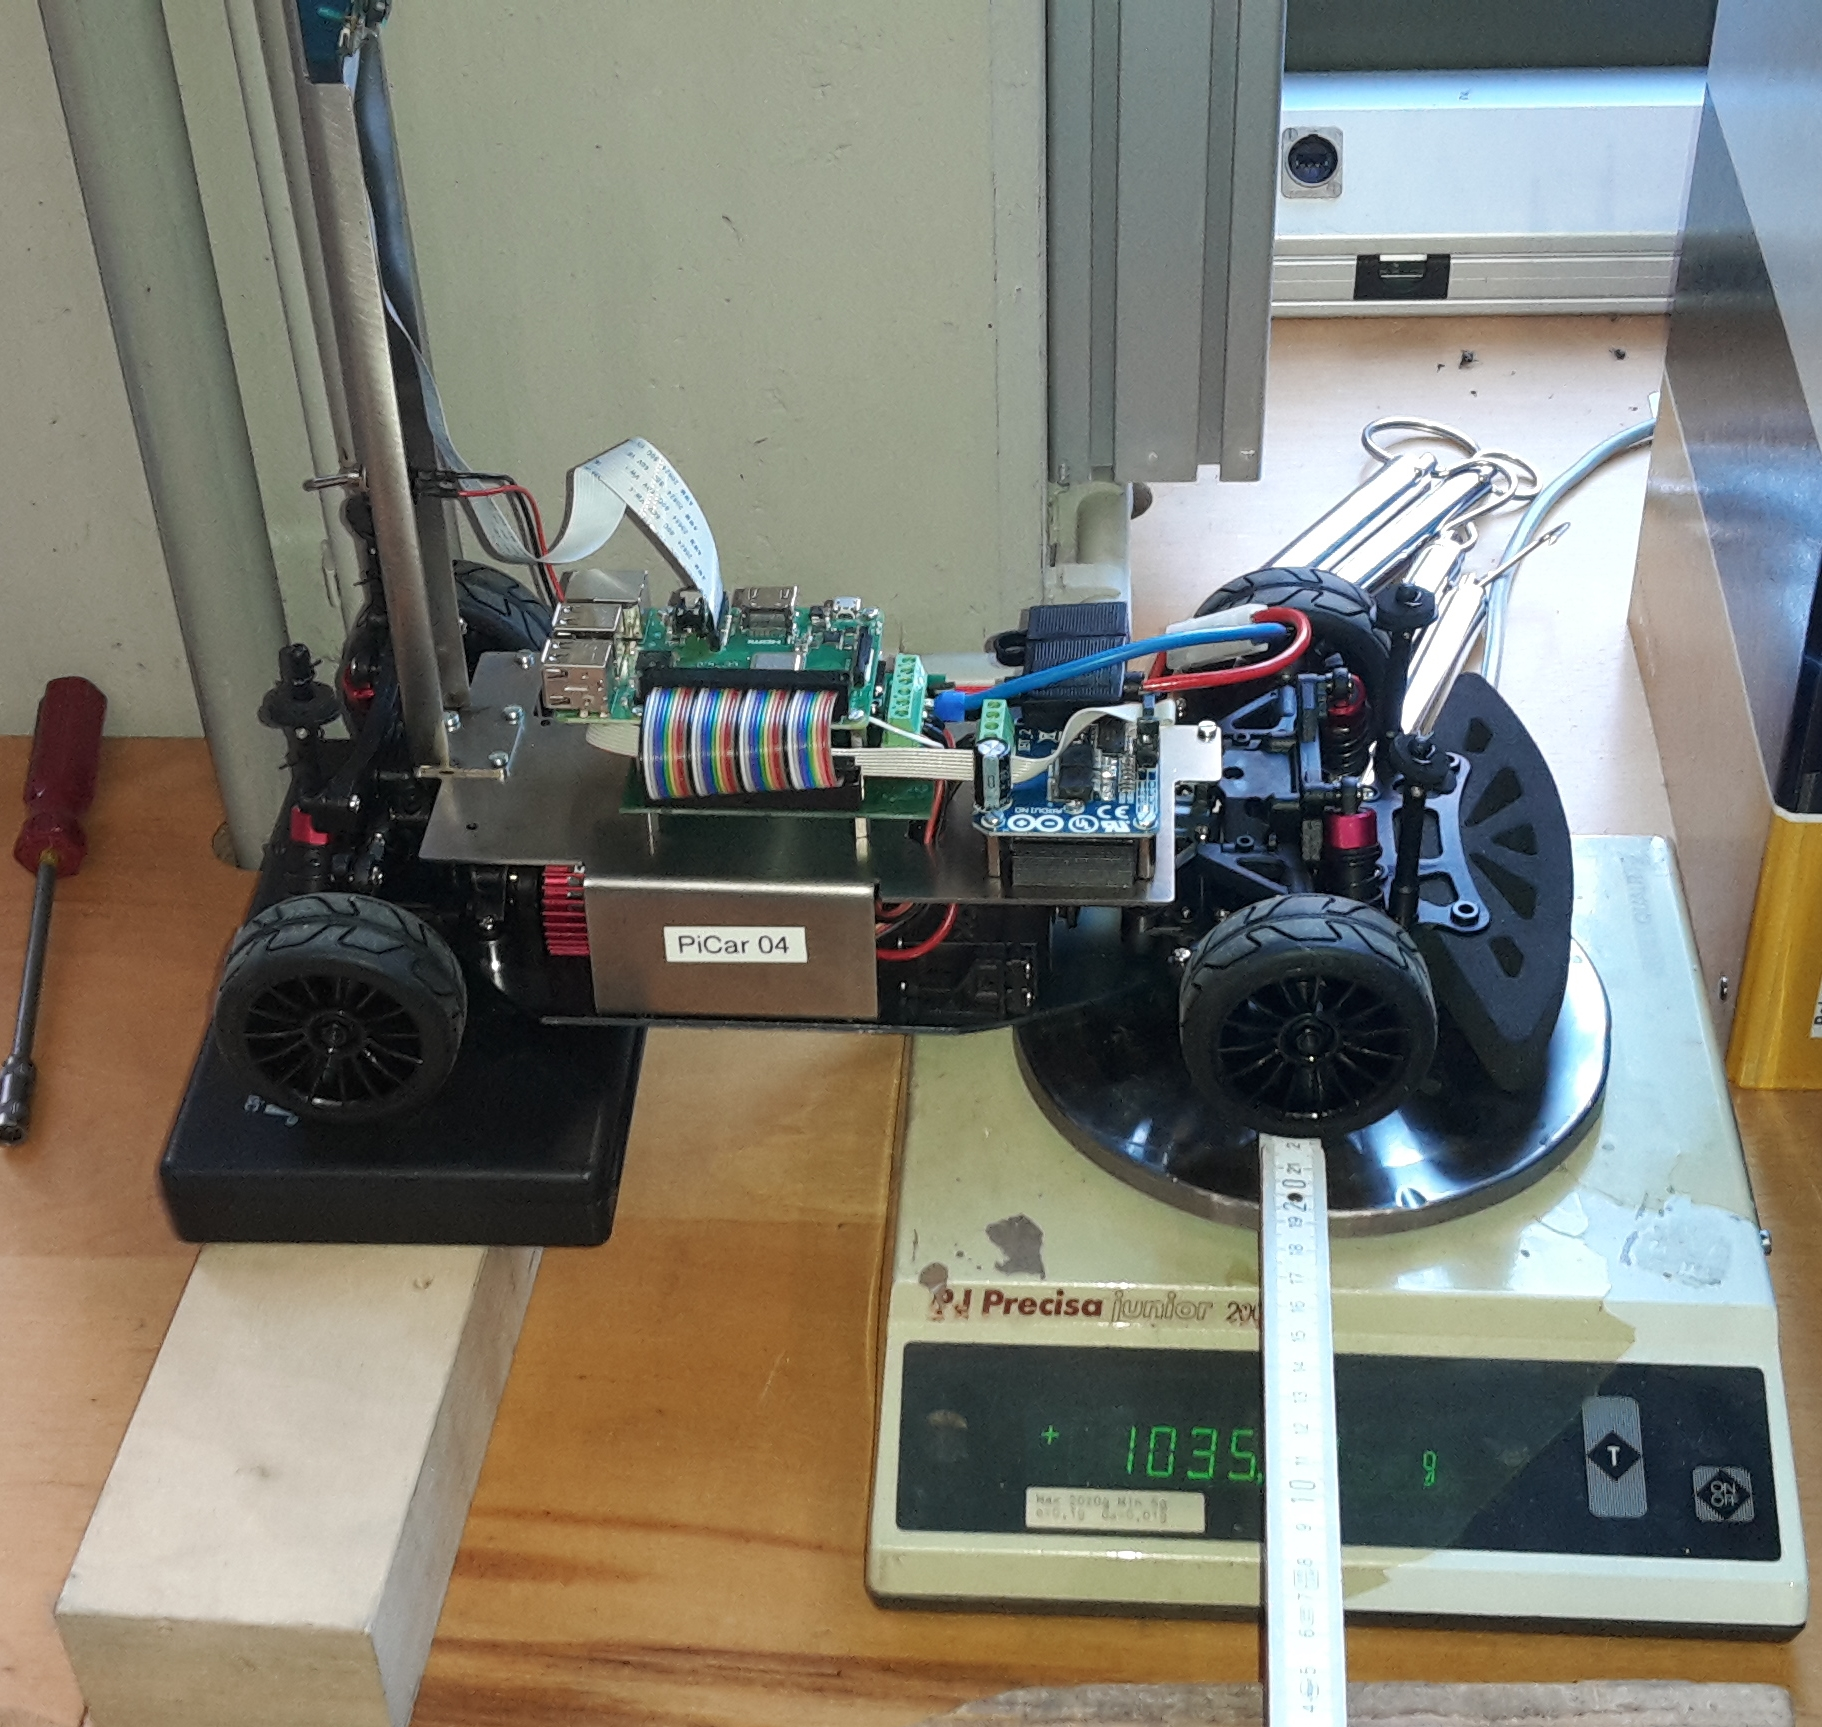
\includegraphics[width=0.3\textwidth]{Figures/Schwerpunktmessung_vorne_hinten.jpg}
\caption{Versuchsaufbau zur Schwerpunktsbestimmung}


\label{fig:Schwerpunkt}
\end{figure}
Die Schwerpunktslage $x_S$ in $x$-Richtung, bzw. $y_S$ in $y$-Richtung errechnen wir mit den Formeln 

$$x_S = \frac{F_\hi}{F_\hi + F_\vo} l_x, \qquad y_S = \frac{F_\li}{F_\li + F_\re} l_y.$$

Wobei die $x$-Achse parallel zur Längsachse und die $y$-Achse parallel zu den Radachsen des Autos verlaufen soll. $F_\hi$ ist die Kraft, die auf die hinteren Räder auf das Auto wirkt, $F_\vo$ ist die Kraft auf die vorderen Räder und $l_x$ ist die Länge zwischen den Radachsen. Entsprechend sind $F_\li$ die Kraft links, $F_\re$ die Kraft rechts und $l_y$ die Länge zwischen den Rädern, wobei wir mit links in Fahrtrichtung links meinen. \\
Um die Kräfte zu bestimmen, haben wir zunächst das Gesamtgewicht $m$ des Autos mit der bereitgestellten Waage gemessen, wobei wir davon ausgehen, dass die Waage das Gewicht mit vernachlässigbarem Fehler anzeigt. Anschließend haben wir für $x_S$, wie in Abbildung \ref{fig:Schwerpunkt} gezeigt, versucht, nur das Gewicht jeweils vorne und hinten zu bestimmen. Um das Auto möglichst gerade auf die Waage zu stellen, haben wir uns mit einer Wasserwaagenapp auf einem Smartphone und einigen Gegenständen beholfen, was man auch in Abbildung \ref{fig:Schwerpunkt} sieht. Bei diesem Aufbau verlassen wir uns auf die Genauigkeit der App, sowie der möglichst exakten Platzierung des Autos auf der Waage.  
Dabei haben wir die Resultate 

$$ m = 2260.1 \gr,\quad m_\vo = 1035.08\gr, \textnormal{ und } m_\hi = 1230.5\gr$$

ermittelt. Es muss $m = m_\vo + m_\hi$ gelten, nach unseren Messungen erhalten wir aber $m_\vo + m_\hi = 2265.58 \gr$, ein Fehler, der weniger als $1\%$ des Gewichts des Autos ausmacht.
Die Länge $l_x$ zwischen den Achsen beläuft sich auf $l_x = 0.261 \m$, mit der obigen Formel erhalten wir also 

$$x_S = \frac{1035.08 \gr\cdot 9.81 \frac{\textnormal{m}}{\textnormal{s}^2} \cdot 0.261 \m}{2260.1 \gr \cdot 9.81 \frac{\textnormal{m}}{\textnormal{s}^2} } = 0.1195 \m $$

in Relation zur hinteren Radachse. Ganz analog ermitteln wir $y_S$ in Relation zum linken Rad:

$$ m_\li = 1090.0 \gr, \; m_\re = 1158.85 \gr,\; l_y = 0.165 \m 
 \Rightarrow y_S = \frac{1158.85 \gr \cdot 9.81 \frac{\textnormal{m}}{\textnormal{s}^2} \cdot 0.165 \m}{2260.1 \gr \cdot 9.81 \frac{\textnormal{m}}{\textnormal{s}^2} } = 0.0846 \m$$

Auch hier erhalten wir mit $m_\li + m_\re = 2248,58 \gr$ einen Fehler, der $1\%$ des Gesamtgewichts des Autos nicht überschreitet. Zusätzlich haben wir als Kontrolle versucht, das Auto auf einer Stange zu balancieren, und bekamen einen Schwerpunkt heraus, der sich sehr nahe dem errechneten Schwerpunkt befindet.
